% !TEX root =  ./main.tex

\section{Encoding of RS in GT}\label{sec:RS2GTS}

Instead of BioResolve, we can alternatively use graph transformation to generate the underlying LTS of a given Reaction System, on the basis of a start graph (plus dedicated specialised type graph) obtained by transformation from the RS specification. What's more, we can analyse the outcome by building the \emph{occurrence graph} of a given trace, which contains all the rule occurrences and entity instances present in that trace --- anaogous, in fact, to the way a \emph{Petri net process} captures a particular behaviour of a Petri Net. Moreover, if a trace leads to the state in which an undesirable entity is present (for instance, the $\anger$ entity in our toy example), we can also \emph{prune} the occurrence graph, again using graph transformation, to filter those rule occurrences and entity instances that directly contributed to the existence of the undesirable entity.

This leads to the tool chain depicted in \Cref{fig:chain}, the steps of which will be explained in some more detail in the remainder of this section.

\begin{figure}
\centering
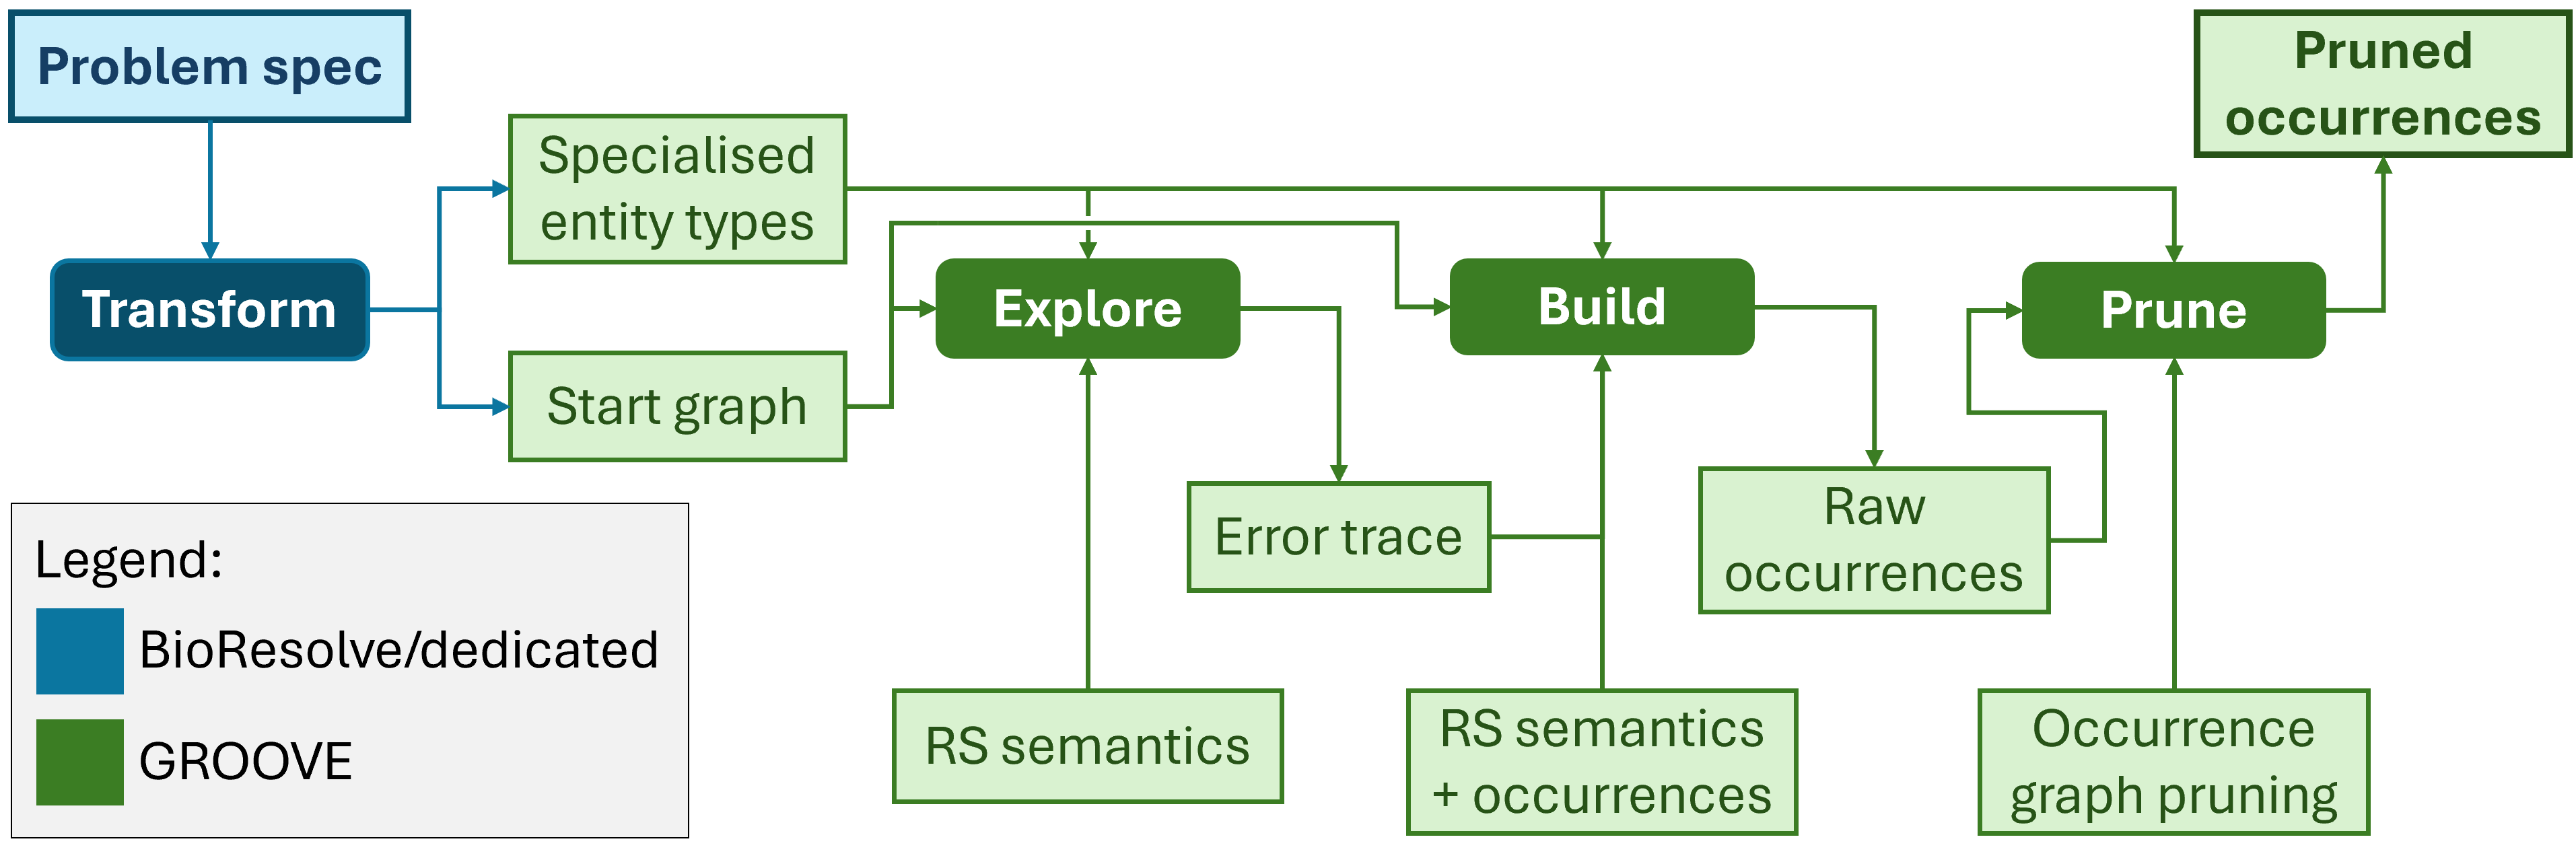
\includegraphics[scale=.25]{figs/chain}
\caption{Reaction System exploration and analysis using \GROOVE}
\label{fig:chain}
\end{figure}

\medskip\noindent\textbf{Transform.}
%
The first step is a text-to-model transformation from a problem specification in \BioResolve syntax into \GROOVE syntax. It produces two artifacts: firstly, an additional type graph, on top of the onee shown in \Cref{fig:core-type}, in which all entities in the problem at hand are provided with their own type (essentially for performance reasons: it speeds up the matching step of \GROOVE); and secondly (more importantly) a start graph in which the entire BioResolve system is encoded as suggested by \Cref{fig:core-type}. For the example system, the additional types as well as two fragments of the start graph are shown in \Cref{toy}.

\begin{figure}
\centering
\subcaptionbox{Spacialised entity types}{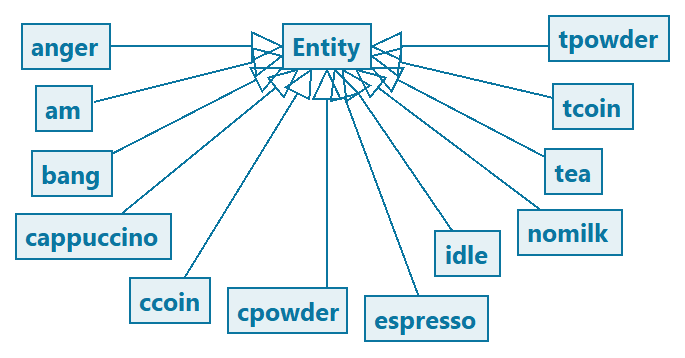
\includegraphics[scale=.2]{figs/toy-type}}
\subcaptionbox{Start graph: Three of the reactions}{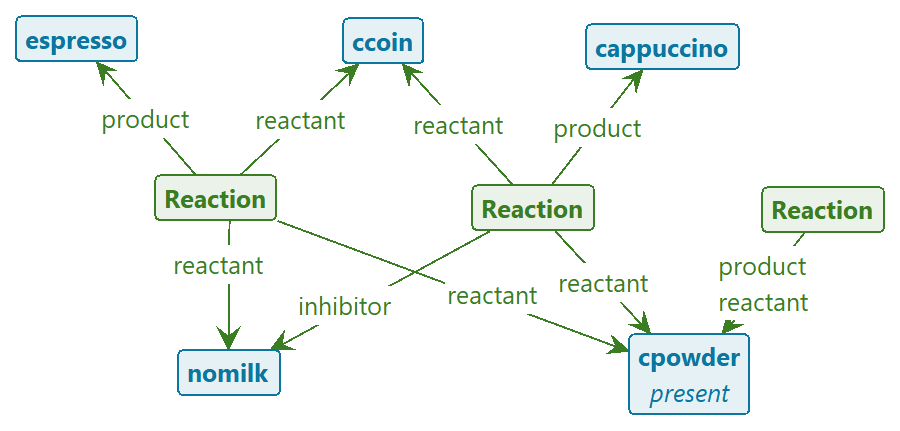
\includegraphics[scale=.2]{figs/toy-reactions}}
\subcaptionbox{Start graph: The \textsf{Student} context process}{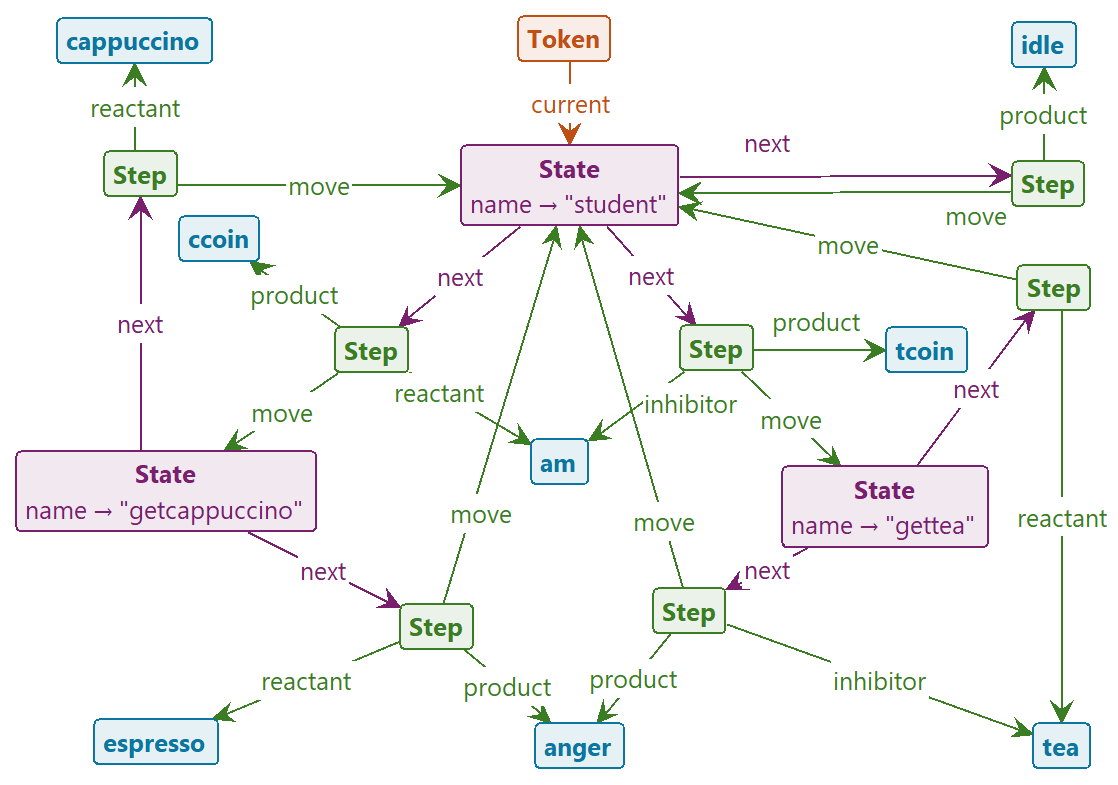
\includegraphics[scale=.2]{figs/toy-context}}
\caption{Graph representation fragments}
\caption{fig:toy}
\end{figure}

\medskip\noindent\textbf{Explore.}
%
The reaction system semantics is encoded in a combination of two rules, which are scheduled to fire in alternation: one encodes the simultaneous firing of all context processes (involving a nondeterministically selected enabled \Step from every \State with a \Token), and the other encodes the simultaneous firing of all enabled \Reaction{}s, while simultaneously erasing all \Entity{}s that were not just produced. The production or erasue of an \Entity is encoded the creation or deletion of a \present flag on a permanently existing \Entity node, \emph{not} by the creation or deletion of the node itself. In addition, to keep track of which nondeterministic choices were actually taken, the context rule marks the \Step{}s that were selected with a \fired flag, which is erased by the reaction rule.

\begin{figure}
\centering
\subcaptionbox{Spacialised entity types}{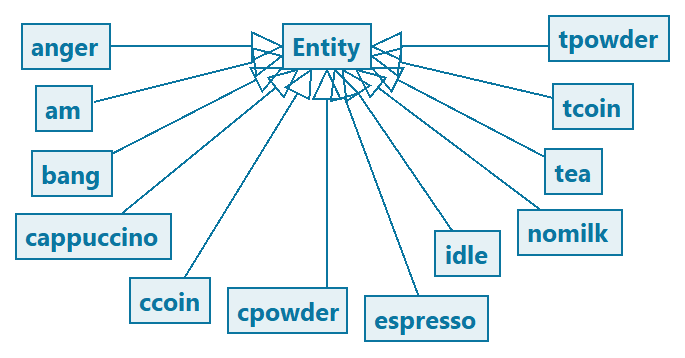
\includegraphics[scale=.2]{figs/toy-type}}
\subcaptionbox{Start graph: Three of the reactions}{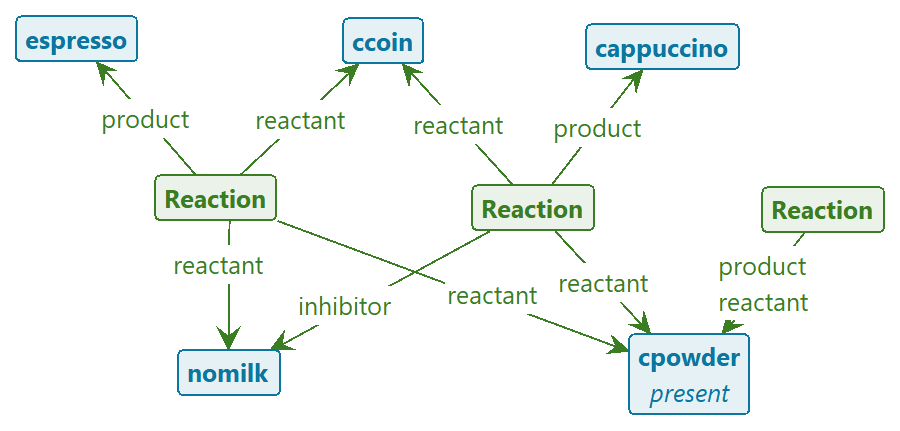
\includegraphics[scale=.2]{figs/toy-reactions}}
\subcaptionbox{Start graph: The \textsf{Student} context process}{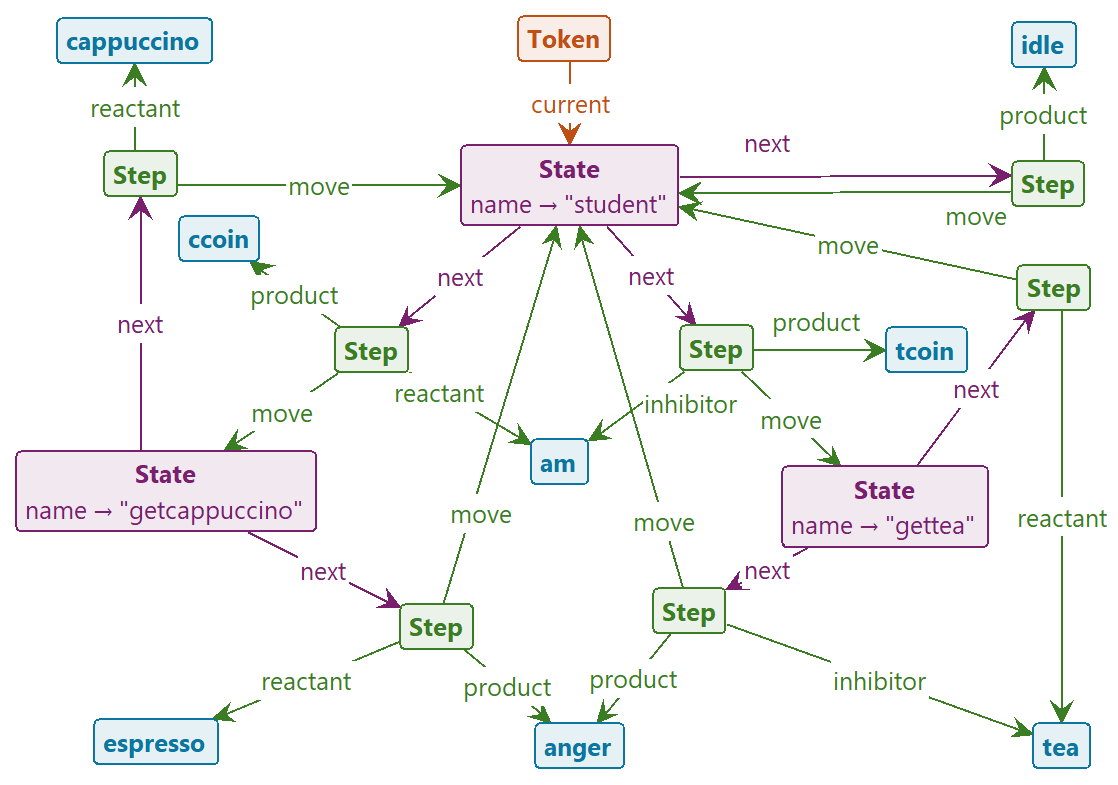
\includegraphics[scale=.2]{figs/toy-context}}
\caption{Graph representation fragments}
\caption{fig:toy}
\end{figure}


\medskip\noindent\textbf{Build.}
%

\medskip\noindent\textbf{Prune.}
%


\begin{quote}\it Notes:
\begin{itemize}
\item Rules for implementing RS semantics
\item Conversion of a trace to a control program
\item Using recipes in the occurrence graph building
\end{itemize}
\end{quote}